\section{Introduzione}

La modellazione generativa può essere definita come segue:
\begin{quoting}
        “La modellazione generativa è una branca del machine learning che prevede l'addestramento 
         di un modello per generare nuovi dati inediti, che sono correlati all'insieme di dati 
         di addestramento originale.”(David Foster, $2023$~\cite{fosterGenerativeDeepLearning2023})
\end{quoting}
    

\noindent Si consideri, ad esempio, un insieme di dati (\emph{dataset}) che annovera immagini di chitarre. È possibile \emph{addestrare} un modello generativo su tale dataset
per desumere le regole che governano le complesse relazioni sussistenti tra i pixel nelle immagini delle chitarre.
A valle della fase di addestramento, avvalendosi del suddetto modello, è possibile creare nuove immagini inedite di chitarre
che non erano presenti nel dataset di partenza (Figura~\ref{fig:gen_model}).



\begin{figure}
        \centering
        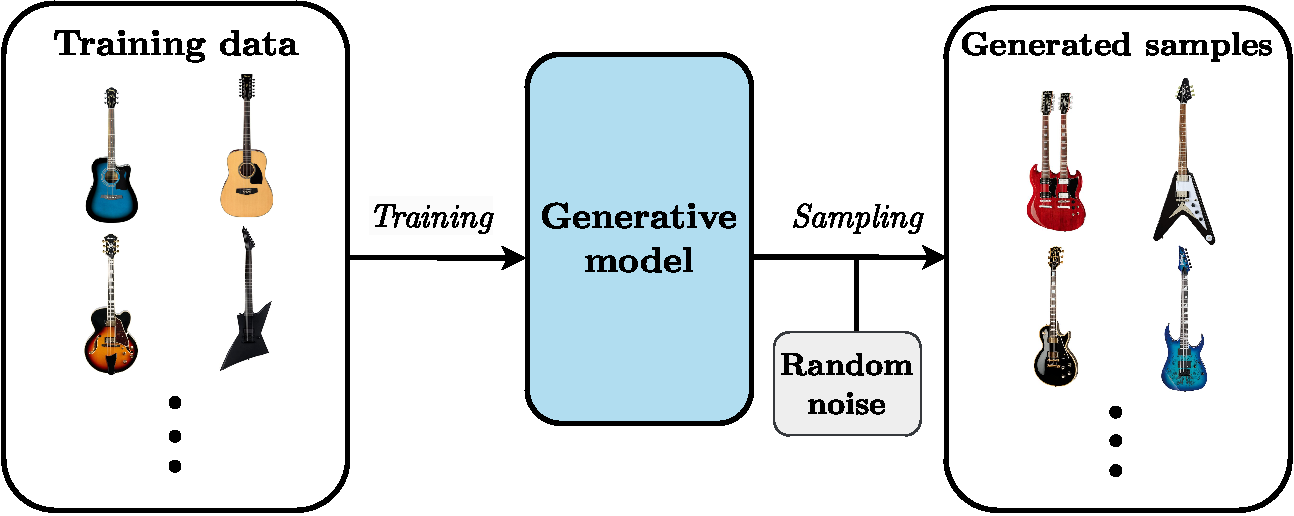
\includegraphics[keepaspectratio, scale=0.55]{Generative_model}
        \caption{Esempio di modello generativo. Fonte:~\cite{fosterGenerativeDeepLearning2023}.}
        \label{fig:gen_model}
\end{figure}



\noindent È importante osservare che un modello generativo è intrinsecamente \emph{probabilistico}. Infatti 
la peculiare capacità di un modello generativo di produrre dati inediti
sottende l'apprendimento della distribuzione incognita dei dati di addestramento, 
cosicché \emph{campionando} da tale distribuzione sia possibile generare nuove istanze di dati: ciò richiede una certa variabilità e incertezza.


Qualora il modello fosse scevro da qualsivoglia elemento di aleatorietà 
(e.g.\ il modello è semplicemente un calcolo fisso, come prendere il valore medio di ogni pixel nel set di dati,~\cite{fosterGenerativeDeepLearning2023}),
stante la sua natura deterministica, non sarebbe generativo.   